\documentclass[nobiblatex]{LTHthesis}
\usepackage[T1]{fontenc}
\usepackage[utf8]{inputenc}
\usepackage{mathptmx, helvet}
\usepackage{xfrac}
\usepackage[left=2.5cm,right=2.5cm,top=3cm,bottom=5cm]{geometry}
\usepackage{graphicx}
\usepackage{listings}
\usepackage{url}
\usepackage{verbatim}
\usepackage[]{algorithm2e}
\usepackage{lipsum}
\usepackage{titlesec}
\usepackage{todonotes}
\usepackage{framed}

\newcommand{\martina}[1]
  {\todo[inline,color=red!30,caption={}]{\textbf{Martina:} #1}}

\newcommand{\fixed}[1]
  {\todo[inline,color=blue!30,caption={}]{\textbf{Fixed:} #1}}

\begin{document}
\begin{titlepages}
\author{Fredrik Johnsson and Olle Svensson}
\title{Resource management and prioritization in an embedded Linux system}
\year{2014}
\month{June}
\TFRT{9999}  %%  You will get the number from the department.
\printer{Media-Tryck} %% You may get other information from the department.

\end{titlepages}
\setcounter{page}{1}
\pagenumbering{roman}

\chapter*{Abstract}

This master thesis tackles the problem of limited computing resources on a
camera that is executing computing applications together with image
acquisition and streaming. The thesis was carried out at Axis Communications
in cooperation with the Department of Control at Lunds University. The
problem of limited resources on an Axis camera is handled by a two part
solution where a resource manager (RM) distributes the available resources
and services can adapt their service level (SL) in order to finish their
jobs on time. The solution is based on game theory, where services are
players, varying their service levels in order to get a good match between
given resources and their computing requirements. This service level
adaptation scheme is partially implemented for the streaming service on the
camera and for some test services, performing mathematical operations. The
resource manager is incorporated into \texttt{systemd}, and uses 
\texttt{cgroups}~\cite{cgroups} to distribute the computing capacity.
\martina{Add one sentence to summarize the results.}


\chapter*{Acknowledgements}

We want to thank our supervisors, Umut Tezduyar-Lindskog, Axis and Martina 
Maggio, LTH Department of Control. We would also like to thank engineering 
manager Pontus Bergendahl, Axis.

\newpage

\tableofcontents
\newpage

\setcounter{page}{1}
\pagenumbering{arabic}

\chapter{Introduction}

This master thesis treats the problem of assigning limited resources to
embedded cameras. Axis cameras are used for the study. Axis is a company
founded and based in Lund that manufactures network relayed surveillance
cameras and video encoders.

\section{Problem formulation}

To save energy and make better use of the available hardware, there is a
trend to have multiple resource intensive applications running on Axis
cameras. These applications are \emph{services}, that should execute within
a certain time and with variable precision requirements. At the same time,
reliable and consistent video frame rate and quality is a necessary
condition to be fulfilled, which calls for running video streaming
services in isolation, without being subject to the interference of
other services. The two conflicting requirements make different services 
compete for resources like CPU and RAM. This may result in poor performance 
of the camera, when the execution scenarios bring the camera under a load
that is heavier than the usual design one. For example, when answering calls
from the network, the camera is subject to a heavier demand. 

In this scenarios it would be advisable to have a technique to diminish
the load produced by services that are not necessary, ideally without
affecting their timing properties. The quality of service reduction is
often addressed via the introduction of service levels, where services can
decrease the load generated on the hardware by lowering their service level,
therefore producing results that have a lower quality. When the load
conditions are back to optimal, the service can increase the service level,
to provide the best available quality without harming the execution of the
most important applications.

This work implements a game theoretic mechanism based on the Game Theoretic 
Resource Manager (GTRM), developed at Lund University~\cite{gtrm} and a
library that lets services implement the service level adaptation and the
communication with a global resource manager. The goal is to demonstrate
that it is possible to use GTRM on an Axis cameras running Linux and to use
it to manage applications competing for resources. The evaluation features
the streaming application, competing with load generators. The image quality
is taken as the service level and the cameras are assumed to have a desired
frame rate, therefore introducing for each frame a deadline of 
\(1/desired framerate\).

\section{Related Work}

The problem of allocating resources to running applications and at the same
time varying the quality of the computation of these applications to avoid
overload conditions has been addressed in many different ways, sometimes
also using game theory.  

For example, Wei et al.~\cite{Wei10} have used game theory to assign
resources to fully parallelizable tasks. Contrary to their approach, in our
case applications are not fully parallelizable and could execute sequential
sections. In some of these sections, assigning more resources would not
speed up the application, while in others the benefits will be significant.
The resource manager developed in this thesis, therefore, needs to act based
on actual measurements.

Subrata et al.~\cite{Sub08} solved the problem of balancing the load in grid 
computing by applying game theory. Here the players are machines that wants 
to maximize their profit by finishing jobs that arrive according to a 
Poisson process. Grosu and Chronopoulos~\cite{Gro05} made similar work with 
load balancing strategies. The load is distributed amongst different 
competing players which would hopefully reach a common state which would 
benefit all the players the most. However, the is no cooperation on the
application side to reach a consensus.

Many resource managers are feedback oriented. The first resource managers
that make explicit use of control theory and feedback loops was developed 
by Lu et al.~\cite{LuS99a}, Steere et al.~\cite{Ste99} and Eker et 
al.~\cite{Eke00}. However they do not implement the concept of varying the
computation quality, or service level.

The QoS-based Resource Allocation Model (Q-RAM) was proposed by Rajkumar et 
al.~\cite{Raj97a} for managing of multidimensional resources. Here it is 
desired to minimize the QoS constraints while maximizing the total 
utility. The solution is centralized and every application receives a
certain quality to be used for the computation and cooperate with the
architecture by enforcing that quality. However, the amount of communication
needed to achieve this goal is non-negligible and therefore it is not
advisable for a video surveillance and streaming systems where the network
bandwidth is used to stream the surveillance videos.
 
A solution that both manages the resources and the service level of an 
application is proposed in the ACTORS project~\cite{Bin11}, but just as the 
solutions proposed by \cite{Raj97a,Soj11,Arz11} the solution is centralized. 
Separating the service-level adjustment and the resource management has been proposed in the context of network bandwidth allocation~\cite{Sil11}.

GTRM~\cite{gtrm}, that is used here as a reference point, decouples the
resource assignment and the service level selection, but it is implemented
with \texttt{SCHED\_DEADLINE}, which is not included in the Linux kernel
used for Axis cameras. Moreover, Axis cameras are already exploiting the
resource allocation capabilities offered by \texttt{systemd}. In this
work, a GTRM-like approach is implemented to be applicable to Axis cameras.

\section{Outline}

The remaining of this report is organized as follows.

\begin{itemize}
\item Chapter~\ref{chp:background} gives a detailed description of
  the software and hardware used during this project.


\item Chapter~\ref{chp:development} details the implementation and design
  decisions, defining therefore how the resulting camera acts.
\item Chapter~\ref{chp:usecases} discusses the use cases that where
  taken as a reference for the project. These describe the product
  functionality and are relevant to test the resulting prototype.
\item Chapter~\ref{chp:test} outlines how the product was tested.
\item Chapter~\ref{chp:results} shows the results obtained with the
  tests and discusses the findings of the thesis.
\item Chapter~\ref{chp:conclusion} finally concludes the report and
  highlights future works.
\end{itemize}



\chapter{Background}
\label{chp:background}

\section{Game Theoretic Resource Manager}

The aim of the resource manager is to make sure that the running applications
have acceptable performance levels. The decision about how much resource to
allocate to each application is based on its performance. The applications
performance are measured in terms of \emph{matching functions}, that is how
good is the match between the resource given to the application and the
corresponding deadline. The assumption behind this is that the resource
distribution determines the execution time to complete a job. The applications
are supposed to be made of jobs. 

The matching function, is calculated as the difference between the
applications deadline and the execution time of the jobs. Ideally the matching
function should be zero. When zero, the application has just enough resources
to meet its deadline running with some service level. When positive, the
resources are abundant to execute the jobs timely, indicating that the job
is done before deadline. A negative matching function means that too little
resource is assigned, indicating that the application has missed or will miss
its deadline.

The framework consists of two parts: the service level adaptation and the
resource management. These two parts are independent and decoupled.

\subsection{Service Level adaptation}

The Service Level (SL) defines the quality of the service provided by the 
application. In the case of the streaming application, the service level
is defined as the quality of the image to be streamed, but for a different
application, the service level can mean something else. The main property of
the SL is monotonicity. An increase in SL gives an increase in the required
resource on the application's side. The idea is to change the SL to optimize
the utilization of the amount of resources available. 

When the performance is too low, the application is supposed to decrease its
service level, while when the performance is too high, the application will
increase the quality of the performed computation. This will make sure that
the application is always presenting valid result in time but with varying
quality, as a trade-off. This adaptation is done by the application itself,
without the resource management policy interfering with it.

\martina{You should write a paragraph with an example on how the service
  level is adjusted. For example, when you take the \emph{test application}
  what is the service level? Is it the same as the test application of
  the original GTRM? If so, write it and write \textbf{how} the adaptation
  is performed: for example, every 10-th jobs? What is a job? What is the
  equation behind the adaptation. You should also clarify that it uses
  the matching function as well (if it does it) --- in the original GTRM
  contribution it was using the performance multiplier, which is a variation
  with respect to the original performance measurement.}

\subsection{Resource Management}

The Resource Manager (RM) measures the performance of the applications. It
tries to distribute the resources in the best possible way to the running
applications, for them to meet their performance requirements. The resources
are modeled as ``virtual platforms''. A virtual platform represents a
percentage of the total available resources; for example, the amount of time
an application is allowed to use the CPU with respect to the other 
applications. Here ``resources'' could refer to something rather than CPU,
such as memory or network bandwidth, depending on what is allocated in the
system.

\martina{Write the equations for the resource adaptation. Take them from the
  ECRTS paper. Describe when the resouce manager acts. Is it every second?
  Are there events that triggers it? For example, when a new application is
  introduced, what happens?}

\begin{equation}
adaptation
\label{eq:resourceadaptation}
\end{equation}

\subsection{Decoupling}

The theory behind the decoupling of the resource allocation and the service
level assignment was developed at the Department of Automatic Control at
the Lund University. The resulting resource manager is referred to as Game 
Theoretic Resource Manager (GTRM).

Decoupling the two adaptations makes it possible to obtain a linear time
complexity for the resource adaptation algorithm. In fact, the amount of
operations that are necessary to perform the adaptation defined by
Equation~\eqref{eq:resourceadaptation} depends only on the number of
running applications. Also, one of the main benefits of this decoupling is
that the task of adjusting the SL is given to the applications that have
knowledge of how to tune their parameters in order to adjust them to their
needs, to the amount of resource received and to the quality of the 
computation.

\section{Systemd and Cgroups}

Systemd [sysd] is a daemon for Linux, that executes system management
operations. It is the first process that starts during boot, and thus it is
given the PID 1. Systemd implements a lot of features for increased
performance and system management over previous start up processes, like
initd. It also has different features for management of resources, using
cgroups~\cite{cgroups}, which makes it interesting for a resource manager
implementation. 

Cgroups~\cite{cgroups}, abbreviated from control groups, can be used to set
the amount of resources, such as CPU or memory, of a process or a group of
processes via a virtual file system. This file system forms a tree where the
resources of a parent folder are shared by its children. The division of the
resources among the children are determined by the amount of ``shares'' the
children has been given. 

\begin{figure}[t]
\centering
\begin{picture}(170,170)
\put(95,130){\framebox(40,30){CPU}}
\put(115,130){\line(-2,-1){40}}
\put(115,130){\line(2,-1){40}}
\put(55,80){\framebox(40,30){Slice 1}}
\put(135,80){\framebox(40,30){Slice 2}}
\put(75,80){\line(-2,-1){40}}
\put(75,80){\line(2,-1){40}}
\put(15,30){\framebox(40,30){Service 1}}
\put(95,30){\framebox(40,30){Service 2}}
\end{picture}
\caption{The slices and services in the cgroup tree.}
\label{fig:ctree}
\end{figure}
\begin{figure}[t]
\centering
\begin{tabular}{|c|c|c|} \hline
\textbf{Name} & \textbf{CPUShares} &  \textbf{\% of CPU} \\ \hline \hline
CPU & 1 & 100 \\ \hline
Slice 1 & 400 & 80 \\ \hline
Slice 2 & 100 & 20 \\ \hline
Service 1 & 200 & $2/3 * 80 = 53$ \\ \hline
Service 2 & 100 & $1/3 * 80 = 27$\\ \hline
\end{tabular}
\label{fig:ctable}
\caption{Table over assigned CPU for the different units.}
\end{figure}

Each application can be run as a ``service'' by specifying a service file
which defines many different parameters and options. In this file, it is
possible to specify which application or applications should be associated
with which service and for example how much CPU shall be given to this 
service. The service file can then be placed in a certain folder in the cgroup
file hierarchy, see Figure~\ref{fig:ctree}.

Different folders are used to represent different cgroup controllers or a
combination of controllers. Depending on which controllers are enabled,
some features are available, such as limiting CPU and memory.
Services can be grouped into different slices and share properties depending
on which slice they belong to. One can for example set how much CPU-time 
shall be given to the applications in the slice and decide how the
applications will divide it amongst themselves.

In this implementation of the \emph{GTRM}, the resources are divided using
the CPUShares property of the \emph{slices} or \emph{services}, both special
cases of the base type \emph{units}. Every slice is represented by a folder
in the cgroup tree and has a CPUShares property that decides how much of the
available resources of the parent slice it will get. A slice contains 
services and services contains applications. 

All the resources of a parent slice will be hierarchically divided to the
units that are classified under this slice according to how much shares
each of them has. A unit that has a third of the total shares of all units
on the same level under its parent slice will receive a third of the
resources available for the parent. In case of a multi-core system, the shares are distributed over all the CPU cores. For example if two services are given 100 and 300 CPU-shares respectively, running on a four core system, one service may use 100 \% of one core and the other 100 \% of each of the remaining three cores.

An example of this is shown in 
Figure~\ref{fig:ctree} and Figure~\ref{fig:ctable}. Note that the top 
level folder in this example, the controller named CPU, is alone on its
level meaning that the CPUShares for this slice do not matter since there
is no competition. There are two slices dividing the CPU-controller, the first slice is given four times the amount of CPU-shares compared to the second slice. This means that the applications in slice 1, is assigned 80 \% of the CPU-time in total. The applications running in slice 1 are defined in two services, which also specify the amount of CPU-shares for each service. The first service is given a total of 200 shares and the second 100 shares. Service 1 will thus be given \sfrac{2}{3} of the shares in slice 1 and service 2 the remaining \sfrac{1}{3}.

\fixed{Describe a little bit better the example that you are giving.
  Maybe complete the numerical example of what you would give to each 
  of the slices and to each of the services inside the slices and how 
  would the CPU behave. What do the number in the table mean?}

\fixed{And, if you are in a multicore environment, what happens
  when you setup a slice? On which core is the slice allocated? Is there
  any enforcement that the slice would effectively be respected? Can it
  be split among multiple cores?}

\section{Video Streaming}

The video streaming application is based upon the GStreamer multimedia
framework. The framework is a modular system, where a chain is built by
linking elements together in a pipeline to form a process chain. 
The data flows downstream from a source element, through filter elements 
and end up in a sink element, see Figure~\ref{fig:pipeline} for a graphical
representation of the pipeline. 

\begin{figure}
\begin{framed}
\label{fig:pipeline}
\begin{picture}(100,60)
\put(0,60){Pipeline}
\put(0,4){\framebox(50,50){Source}}
\put(50,29){\vector(1,0){50}}
\put(100,4){\framebox(50,50){filter}}
\put(150,29){\vector(1,0){50}}
\put(200,4){\framebox(50,50){Sink}}
\end{picture}
\end{framed}
\caption{The GStreamer pipeline.}
\end{figure}

The data is contained into buffers. Buffers can contain one or more frames,
flowing downstream. On Axis cameras, the source elements receive the images
already compressed by external hardware through another application which
reads a file descriptor in order to get the frames from the encoding device.
The data is then sent through a number of filters and finally is released to
the network by the sink element. This chain is dynamically created depending
on different settings like codecs used (\emph{jpeg, h264 and more}) or 
network connection (\emph{http or udp}).

\martina{Can you add a couple of information about the processing? How are
  the images being processed? What are those ``filters''? At least in one
  example that is reasonable (choose a codec and a network connection type
  and describe the pipeline in that case).}


\section{Sockets and epoll}

This section introduces ...
\martina{Add a short introductory sentence above. This sentence should
  state why you are introducing sockets and the epoll function.}

\subsection{Sockets}
The communication between applications and \texttt{systemd} is obtained
through sockets. The RM runs in the \texttt{systemd} main loop, therefore
sockets are used to send data between the RM and the applications.

Sockets are the endpoints for \emph{inter-process communication} (IPC) 
flows over a network, where the entities communicating may reside on the
same physical device or are simply nodes on the same network. These sockets
are provided by the \texttt{socket()} system routine in Linux, therefore
their usage is regulated by the normal operating system APIs.

A call to the \texttt{socket()} API function creates a socket and returns 
an integer, a unique \emph{file descriptor} representing the socket for
future usage. A file descriptor in Linux is associated with an open file,
where the file can be anything that can be written to or read from. 
Knowing the descriptor gives read and write access to the socket. 
A socket has a type, being it either \emph{stream} or \emph{datagram}, 
the latter is the one used by the GTRM socket.


\subsection{Epoll}
Epoll is a Linux system call, allowing the user to listen to multiple 
sockets simultaneously. The API function \texttt{epoll\_wait(...)} returns 
a queue of event-objects containing information about what file descriptors
have received datagrams together with other information. By looking at this 
queue the user knows what file descriptor to read with to obtain the newly
arrived data.  

\section{Equipment}
The project involves experiments with two different cameras: the M1033 and 
the P3367, both manufactured by Axis. Both the cameras have \texttt{systemd}
installed, although the P3367 runs a more updated version of it.

\subsection{Axis M1033}

This is a small camera, connected to the network either wired or wireless. 
It supports multiple H.264 streams and Motion JPEG running at a maximum
resolution of 800x600 at 30 frames per second. It has two audio streaming
channels, which means that it can both record and play audio clips. 

\begin{figure}[h]
    \centering
    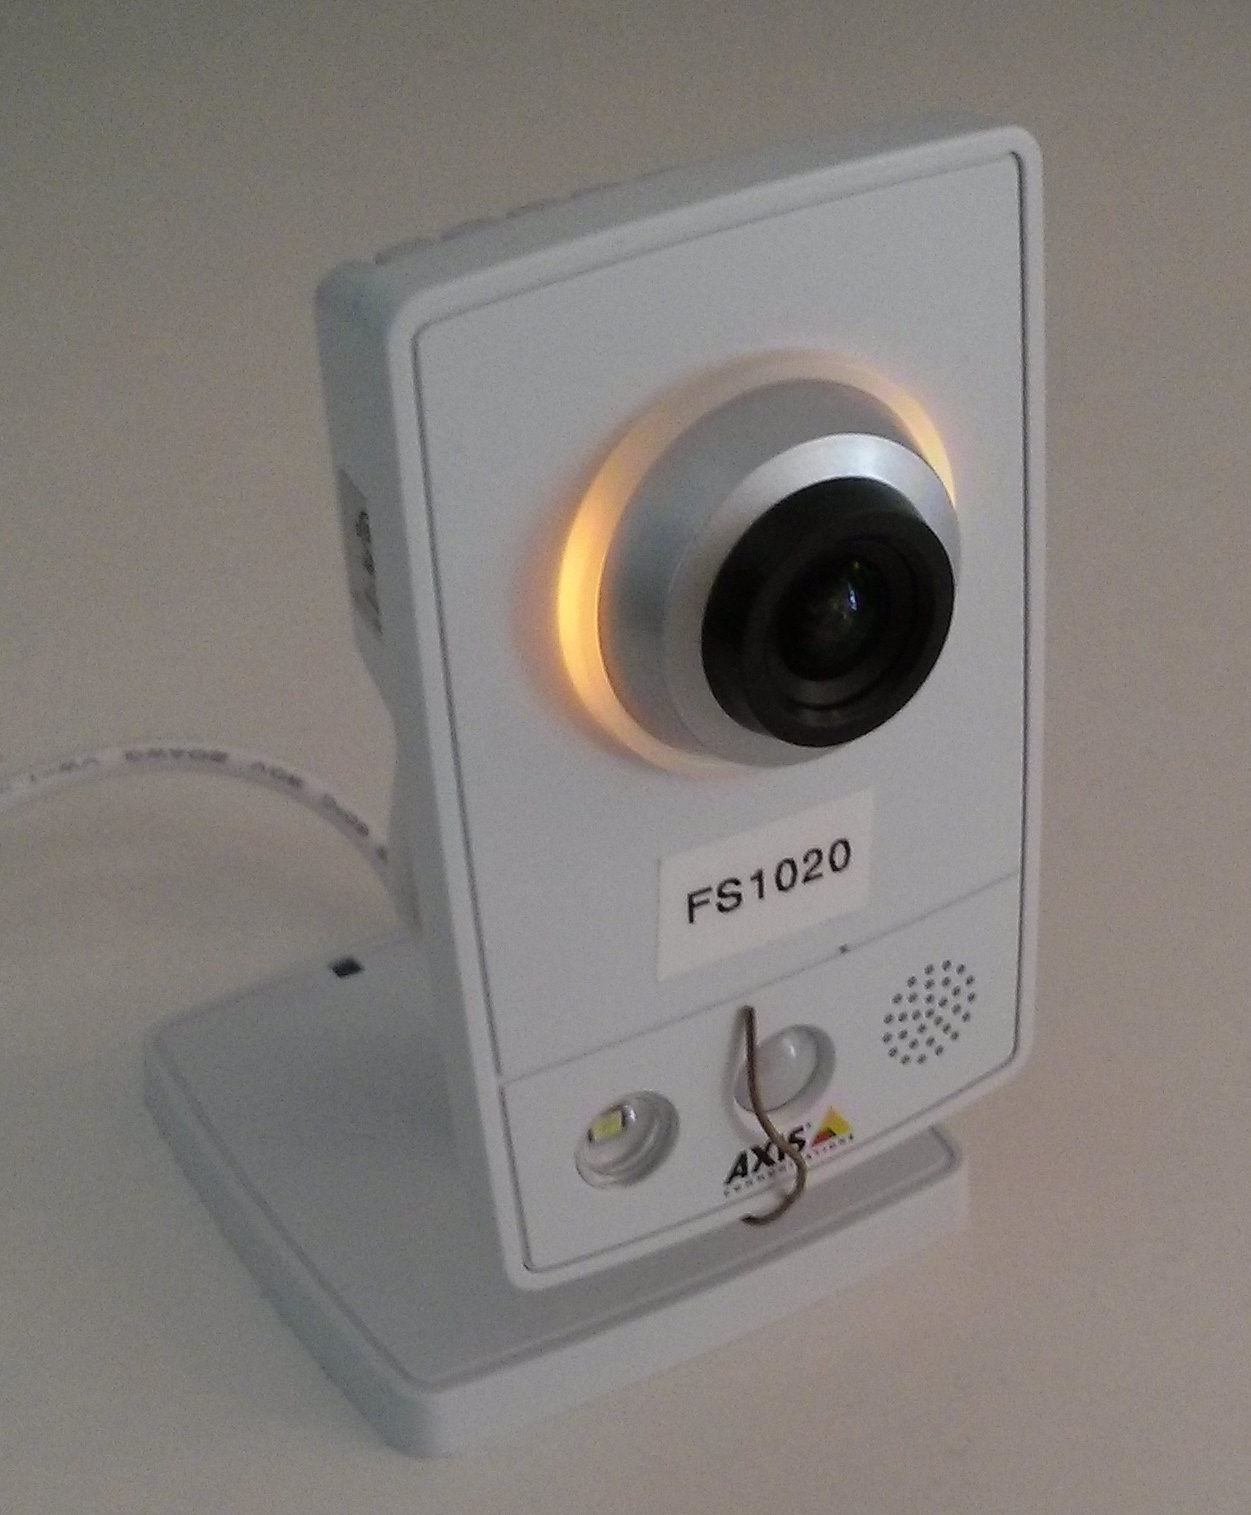
\includegraphics[width=0.5\textwidth]{m1033}
    \caption{The Axis M1033 camera}
    \label{fig:M1033}
\end{figure}

It is very likely, due to its capabilities, that multiple applications run
simultaneously on the hardware, especially due to the ability of recording 
and playing audio clips simultaneously. In fact, while the video is recorded
and sent over the network, it is also possible to run other applications
using the collected data, for example some motion detection application.

\subsection{Axis P3367}

The Axis P3367 is a fixed dome network camera capable of multiple H.264
streams as well as Motion JPEG streams. It supports various frame rates and
resolutions up to 5 Megapixel at 12 frames per second, it also supports 
HDTV 1080p at 30 frames per second and has two way audio streaming 
capabilities.
\martina{dome? home?}

\begin{figure}[h]
    \centering
    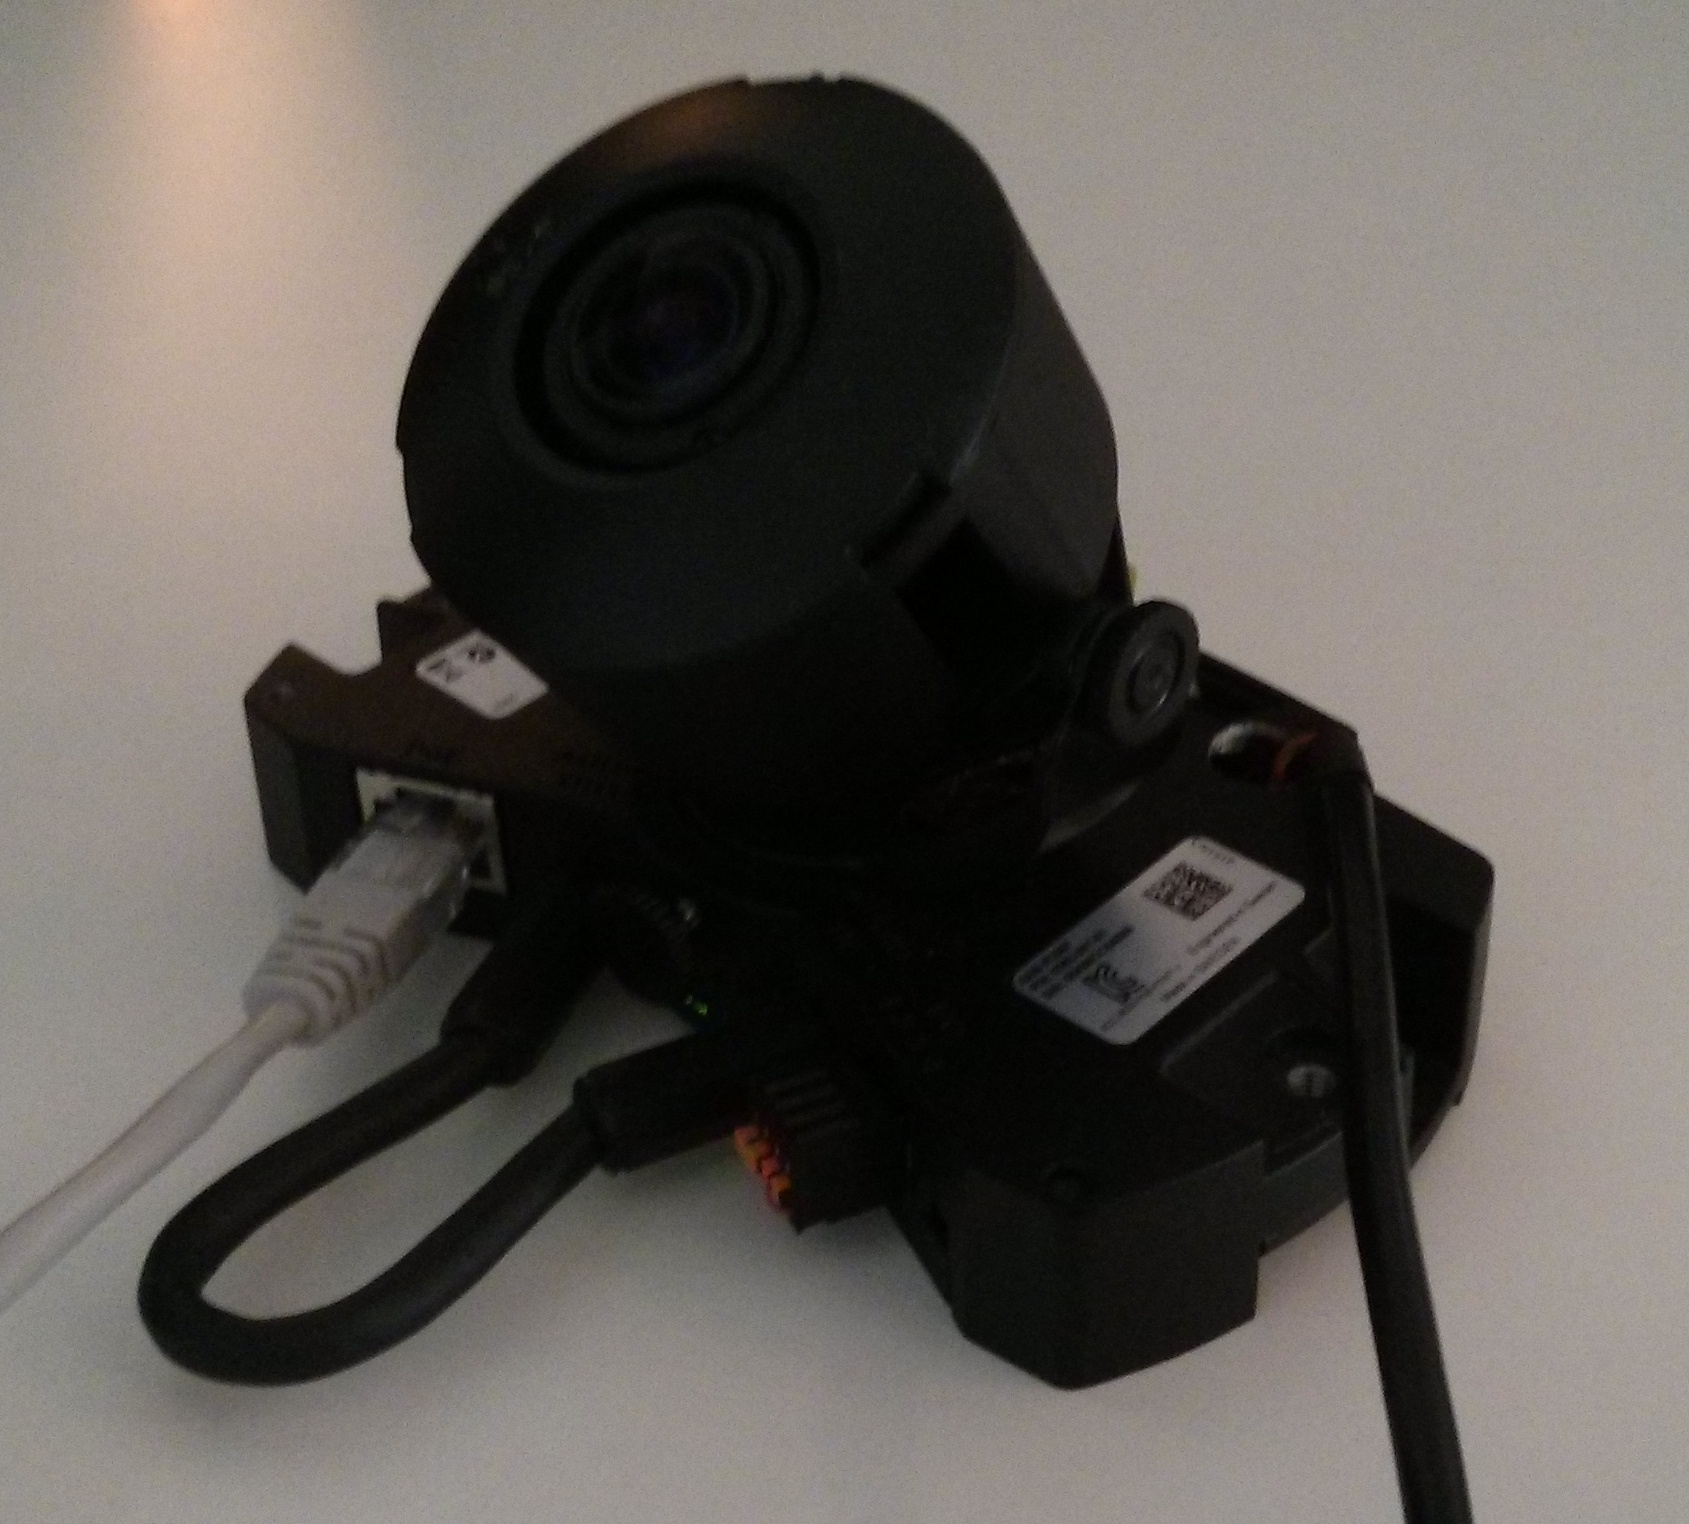
\includegraphics[width=0.5\textwidth]{p3367}
    \caption{The Axis P3367 camera, without its case}
    \label{fig:P3367}
\end{figure}

The power is supplied using Power over Ethernet, therefore the camera does 
not need a separate power supply and is powered directly through the network
cable. It features an ARTPEC-4 system-on-chip, developed by Axis, which
contains a single-core CPU running at 400 MHz and a co-processor dedicated
to video analytics.

It is clearly more advanced than the M1033 but it shares the same
characteristics of being extremely flexible to execute multiple applications
at the same time, especially due to the video analytics co-processor.

\martina{Will you present test with both the cameras or only with one of
  them? Will you present the same tests on both the cameras? In this case,
  explain why one camera is better than another for testing some specific
  feature of your approach. Is there something special beside ``they have
  systemd'' why you chose these two models? How are those positioned
  among the Axis products? Are they in the middle, are they the top of the
  Axis production? What other applications are likely to be run on the
  same hardware? If you have some of the answers to this questions, try
  to insert them in the text.}


\chapter{Implementation}
\label{chp:development}

This chapter describes the implementation of the GTRM framework for
Axis cameras. The code commented upon was written in C and cross-compiled 
using Axis' compiler for the corresponding hardware platform. The resource
allocation framework was testing in different use cases and with a
variety of service files and slices. The resulting plots are generated with
Octave.

\section{Design choices}

Introducing service levels in all the applications running on camera
is not a realistic approach. This is because there are many different
applications, some of which may not even be developed at Axis, and 
developers are not expected to modify all these applications to implement 
the performance measurements and service level features needed, despite the
modification being trivial in many cases. Also, for some applications it is
not possible to identify the concept of service level. 

The service level is in this work implemented for the video streaming
application and for some test application that generates mathematical load
in the system. This thesis only focuses on the implementation of GTRM and 
assumes that a correct implementation of the framework implies also that
the proof of convergence of the game theoretic strategy holds, as
demonstrated for~\cite{gtrm}.

Also, the service level assignment is limited to the linear case, where
resource requirements (in this case CPU requirements) are a linear function 
of the service level. It can be argued that the CPU requirement/SL
relationship can be linearized around a point and hence still considered
linear close to the operating point. 

The matching function used to determine the performance of the application is
time sensitive and reads as
\begin{equation}
f_{i}=\cfrac{D_{i}}{R_{i}}-1
\end{equation}
where $D_{i}$ is the soft deadline for the job and $R_{i}$ is the job 
response time. This matching function is positive when the resource given is
aboundant and negative if it is scarce. It is also zero in case there
is a perfect match between the resource given and the service level set by
the application. The aim of GTRM is to bring $f_i$ to zero for all the
running applications. It is assumed that $f_i$ is measurable also for the
non-service level aware applications. The matching function is updated as
the average of the measured value for the last ten jobs.


\section{Adaptation}

\subsection{Service Level update}
In the following we discuss to possible ways of adjusting the service level.
In the first case, the application only considers information that are
internally available, while in the second case, the application receives
hint from GTRM and follows those hints.

The \emph{independent adaptation} simply multiplies the current service level,
the matching function and a constant scale factor $\epsilon$. This adaptation
decreases the service level if the performance is negative and increases it 
if the matching function is positive. The scaling factor $\epsilon$ slows 
down the adaption rate to avoid instability. 

\begin{equation}
sl_i(t+1)= sl_i(t) + \epsilon*(f_i(t)*sl_i(t))
\end{equation}

The \emph{coordinated adaptation} follows a suggestion given by the resource
manager, that includes also the variation of the resource allocation. In fact,
the resource manager sends to the application a \emph{performance multiplier}
$PM_i$ that is used as an estimation of how much the service levels should
change to match the current allocation, that is unknown on the application
side.

The performance multiplier $PM_i$ is computed as
\begin{equation}
PM_i = (1+f_i) \cdot (vp_i(i+1)/vp(i))
\end{equation}
and the applications sets the new service level as
\begin{equation}
sl_i(t+1) = sl_i(t) + (\epsilon \cdot sl_i(t) \cdot PM_i).
\end{equation}

\subsection{Resource Allocation update}

The resource update changes the virtual platforms allocated to each running
application. It follows the algorithm described in 
``A Game-Theoretic Resource Manager for RT Applications''~\cite[page 4]{gtrm}.

\begin{quotation}
	[...] the RM assigns resources according to the rule:
	\begin{enumerate}
	\item it measures the performance\footnote{As stated in its definition, 
    $f_i$ is a function of the service level $s_i$ and the virtual platform 
    $v_i$. However, here we intentionally hide this dependency and report 
    only the dependency on time $t$, since the RM only measures a value 
    over time.} $f_i(t)$;  
	\item it updates the virtual platform $\tilde{v}_{i}$ as follows:
		\begin{multline}
		  \tilde{v}_i(t+1) = \tilde{v}_i(t) + 
                         \epsilon_{ RM}(t)\Big(- \lambda_i f_i(t) + 
                         \sum_{j=1}^n \lambda_j f_j(t) \tilde{v}_i(t)\Big),
		  \label{eq:RecursionForResources}
		\end{multline}
		where $\epsilon_{ RM}(t)$ is a step-size sequence;
	\item it computes the original value of bandwidth by 
    $$v_i(t+1) = m \tilde{v}_i(t+1),$$
	\item it updates the time $t\leftarrow t+1$ and repeats.
	\end{enumerate}
\end{quotation}

Here $\tilde{v}$ is the normalized virtual platform and $m$ is the number
of computing elements. This means that the computed resource allocation $v$
represents the percentage of the total resources allocated to the application
and is converted into the actual value during the third step of the
algorithm. CPUShares are used here in place of bandwidth.

\martina{Can you comment a bit on what is the difference between CPUShares
  and bandwidth? From what I understand, it makes a difference in the
  multicore case.}

\section{IPC}
The resource management is implemented as a part of systemd, with all of the resource management source code integrated into systemds. If an application has a poor matching function it sends information to systemd via UNIX-sockets. The interprocess communication (IPC) consists of one socket in systemd and one for each application that the RM is monitoring. The socket setup was implemented by more or less copying the “Notify” feature of systemd which is used by certain services that want to for example notify systemd that they have started or about other status changes [sysd-notify].
Systemd uses epoll to find out which sockets has received new messages. The events returned from epoll\_wait() are then put in a prioritized queue. This prioritized queue is then popped and the callback function for top most event is called. This means that a message might not be read immediately after being read from the epoll buffer. Most of the functions used to manage epoll are located in “sd-event”. 


The epoll\_wait function is shown below
\begin{verbatim}


int epoll_wait(int epfd, struct epoll_event *events,
                      int maxevents, int timeout);	 
\end{verbatim}
When there are messages to read on one of the fd:s being watched by the epoll instance referred to by the file descriptor \emph{epfd}, epoll\_wait returns the number of fd:s that have new messages to be read.
The epoll\_event *\emph{events} points to a buffer that will be filled with the incoming events and that will contain a maximum of \emph{maxevents}.
The epoll\_event structure is shown below:

%\verbatiminput{pseudo_epoll.c}

\begin{verbatim}
typedef union epoll_data {
 void    *ptr;
 int      fd;
 uint32_t u32;
 uint64_t u64;
} epoll_data_t;

struct epoll_event {
 uint32_t     events;    /* Epoll events */
 epoll_data_t data;      /* User data variable */
};
\end{verbatim}

The void pointer \emph{epoll\_event.data.ptr} will be set to point to a \emph{sd\_event\_source} structure which is the element that is put in the prioritized queue. This element contains information concerning the prioritization and  defines the event type but also contains a structure containing the fd for the event and the callback function to be used when such an event is received.
In each iteration of the main loop the function \emph{sd\_event\_run} is called, the part of the code that is instructive in this function is shown below:

\begin{verbatim}
_public_ int sd_event_run(sd_event *e, uint64_t timeout) {

struct epoll_event *ev_queue;
unsigned ev_queue_max;
sd_event_source *p;
int r, i, m,timeout;
            
ev_queue = newa(struct epoll_event, ev_queue_max);

m = epoll_wait(e->epoll_fd, ev_queue, ev_queue_max,timeout);

for (i = 0; i < m; i++) {
  if (ev_queue[i].data.ptr == INT_TO_PTR(SOURCE_MONOTONIC))
    r = flush_timer(...);
  else if (ev_queue[i].data.ptr == INT_TO_PTR(SOURCE_REALTIME))
    r = flush_timer(...)
  else if (ev_queue[i].data.ptr == INT_TO_PTR(SOURCE_SIGNAL))
    r = process_signal(e, ev_queue[i].events);
  else if (ev_queue[i].data.ptr == INT_TO_PTR(SOURCE_WATCHDOG))
    r = flush_timer(e, e->watchdog_fd, ev_queue[i].events, NULL);
  else
    r = process_io(e, ev_queue[i].data.ptr, ev_queue[i].events);
}


p = event_next_pending(e);

r = source_dispatch(p);

return r;
}
\end{verbatim}

As can be seen, the \emph{epoll\_wait} function is called and a for loop goes through all of the fd:s and checks what their event type is to call the appropriate function to add them to the prioritized queue.
The gtrm fd is linked to a \emph{IO\_SOURCE} event which means that the function \emph{process\_io()} will be called.

Next the queue is peeked to get the next event in the queue to be dispatched by calling event\_next\_pending():
\begin{verbatim}
	static sd_event_source* event_next_pending(sd_event *e) {
	sd_event_source *p;

	p = prioq_peek(e->pending);
	if (!p)
		  return NULL;

	if (p->enabled == SD_EVENT_OFF)
		  return NULL;
	return p;
	}
\end{verbatim}

Finally the \emph{source\_dispatch} function is called to call the callback function linked to the popped top \emph{sd\_event\_source*} element.

\begin{verbatim}
	static int source_dispatch(sd_event_source *s) {
	int r = 0;

	switch (s->type) {

	case SOURCE_IO:
		  r = s->io.callback(s, s->io.fd, s->io.revents, s->userdata);
		  break;

	case SOURCE_MONOTONIC:
		  r = s->time.callback(s, s->time.next, s->userdata);
		  break;

	case SOURCE_REALTIME:
		  r = s->time.callback(s, s->time.next, s->userdata);
		  break;
	.
	.
	.
		  r = s->exit.callback(s, s->userdata);
		  break;

	case SOURCE_WATCHDOG:
		  assert_not_reached("Wut? I shouldn't exist.");
	}
	
	return 1;
	}
\end{verbatim}  

\subsection{Setting up the socket}

The socket is created and added to the epoll instance in \emph{manager\_setup\_gtrm(...)}, below is the instructive part of the code in \emph{manager\_setup\_gtrm(...)}:




\begin{framed}
		\begin{flushleft}
		
			\textbf{\emph{{static int manager\_setup\_gtrm(Manager *m)}}} \newline
			Used to setup the socket, event source and file descriptor for the resource manager. Called from manager\_startup and manager\_reload.
			\begin{itemize}
			\item m: Reference to the manager.
			\item Return value: Zero if function ran correctly, otherwise it is set to the corresponding error number.
			\end{itemize}
		\end{flushleft}	
\end{framed}







The socket is created in the function  with a call to the socket(..) function.
\begin{verbatim}
fd = socket(AF_UNIX, SOCK_DGRAM|SOCK_CLOEXEC|SOCK_NONBLOCK, 0);
\end{verbatim}

The socket is set to use the protocol family \emph{AF\_UNIX}, which provides efficient communication on the same machine. \emph{SOCK\_DGRAM} sets the socket type to be datagram since there is no need to resend missed obsolete data and no messages are expected to be lost when sent over the same machine anyway. \emph{SOCK\_NONBLOCK} prevents the socket from blocking during a read() call when there is no data to read which should not matter here since the polling makes sure that there is always something to read. A random address name is created and assigned to the socket by a call to bind(). Next the fd for the socket needs to be added to the epoll instance, and an epoll\_event needs to be associated to the fd. The \emph{epoll\_event} contains a pointer to a \emph{sd\_event\_source} that has been described earlier. This is all done in the call:  

\begin{verbatim}
r = sd_event_add_io(m->event, &m->gtrm_event_source, m->gtrm_fd,
 EPOLLIN, manager_dispatch_gtrm_fd, m);
\end{verbatim}

Now the gtrm socket has been added to the poll and a corresponding event will be returned if there is a message on the socket when calling \emph{epoll\_wait(...)}. 
The last thing done in \emph{manager\_setup\_gtrm(...)} is to give the \emph{gtrm\_event\_source} a priority, this affects how the prioritized queue sorts messages from this source type and is set to the same as notify messages.

Once the socket is setup and ready a environmental variable is set in Linux containing the address to the gtrm-socket. This is how applications will know where to send their messages to.


\subsubsection{The callback function for gtrm socket:}
Once an event has been popped from the prioritized queue the callback function \emph{static int manager\_dispatch\_gtrm\_fd(...)} is called. 
The callback function contains all the code that should execute when a message is received on the gtrm socket. The function extracts the data from the message, which is the PID of the sending application, its performance, whether it is satisfied or not and the weight attribute. 
The hashmap, which contains all the applications that are managed by GTRM, is then updated with this new data. 




The instructive parts of the function are shown below:

\begin{framed}
		\begin{flushleft}
			\textbf{\emph{static int manager\_dispatch\_gtrm\_fd(sd\_event\_source *source, int fd, unit32\_t revents, void *userdata)}}\newline
				Called when we receive the performance of an application.
				\begin{itemize}
				\item source: source of the event.
				\item fd: file descriptor to the event source.
				\item revents: Set by the kernel to indicate what event on the file descriptor that triggered the call to this function. In our case it is always the incoming event.
				\item userdata: In this case it contains a reference to the manager.
				\item Return value: Not used, always zero.
				\end{itemize}
		\end{flushleft}	
\end{framed}





First some declarations and initializations

\begin{verbatim}
static int manager_dispatch_gtrm_fd(sd_event_source *source, int fd,
uint32_t revents, void *userdata) {

Manager *m = userdata;    		    
//will contain the read message
char buf[1024];
//will be set to the byte size of the read message
int n;
//will contain the senders adress
struct sockaddr_un *from;
socklen_t fromlen;
//stores RM data about the applications being managed
rm_app_t *app;
rm_app_t *app2;	

fromlen = 1024;
\end{verbatim}

Here the \emph{rm\_app\_t} structure is used:

\begin{framed}
		\begin{flushleft}
			\textbf{\emph{struct rm\_app\_t}}
			Represents an application being managed and consists of the following fields.
			\begin{itemize}
			\item tid: Applications PID.
			\item vp: Virtual platform.
			\item vp\_old: Previous virtual platform.
			\item performance: Performance, or matching function of the application.
			\item weight: The current "weight" of the application.
			\item happy: Indicates if the application is happy with its current performance.
			\item sa: Socket Address, used to send back the performance multiplier.
			\end{itemize}
		\end{flushleft}	
\end{framed}






Now a while loop reads the socket one message each iteration until there are no more unread messages. 

\begin{verbatim}
do{		

	memset(buf,'\0',1023);
	from = calloc(1,sizeof(struct sockaddr_un));
	app = calloc(1,sizeof(rm_app_t));	
	n = recvfrom(fd,buf,1024,0,(struct sockaddr *) from,&fromlen);

	//n is negative if there was no message if socket is non blocking
	n = recvfrom(fd,buf,1024,0,(struct sockaddr *) from,&fromlen);
	if(n<0)
		break;
	if(n>1024){//2do avoid magic numbers
		log_error("manager_dispatch_gtrm_fd:received too big message");
	}	

	gtrm_char2gtrmstruct(buf, app);
	pid_t pid = app->tid;
	app->sa = from;

	if(hashmap_get(m->gtrm_apps, pid) == NULL) {
		hashmap_put(m->gtrm_apps, pid, app);
	} else {
		app2 = hashmap_get(m->gtrm_apps, pid);
		gtrm_update_rm_struct(app,app2);
	}															

}while(n>0);
The callback function which is registered and linked to the events for the gtrm socket when the socket communication is established, contains all the code that should execute when a message is received on the gtrm socket. The function extracts the data from the message, which is the PID of the sending application, its performance, whether it is satisfied or not and the weight attribute. 
The hashmap, which contains all the applications that are managed by GTRM, is then updated with this new data. 
m->update_gtrm = true;

return 0;
}
\end{verbatim}

The data from a message is used to create a \emph{rm\_app\_t} struct. If the hashmap already contains a \emph{rm\_app\_t} struct for the application, the \emph{rm\_app\_t} in the hashmap is updated by calling the function 
\emph{gtrm\_update\_rm\_struct(app,app2)}, otherwise it is added to the hashmap with the application pid as the key.

\emph{gtrm\_lib} functions used above:


\begin{framed}
		\begin{flushleft}
			\textbf{\emph{void gtrm\_char2gtrmstruct(char* str, rm\_app\_t *re)}}
			Extracts data from a received string and store it as a struct instead. The data sent from an application consists of the PID, performance, weight and if the application is satisfied or not.
			\begin{itemize} 
			\item str: String to extract data from.
			\item re: Struct to hold the extracted data.
			\item Return value: None, the result is stored in re.
			\end{itemize}
		\end{flushleft}	
\end{framed}



\begin{verbatim}
void gtrm_update_rm_struct(rm_app_t *src,rm_app_t *dest){
	dest->performance = src->performance;			
}
\end{verbatim}



\subsection{Resource management loop}
The virtual platforms are re-calculated and applied for as long as the applications are not completely satisfied. This is run inside the \emph{manager\_loop}-function in \emph{manager.c}.

\begin{verbatim}
int manager_loop(Manager *m) {
\end{verbatim}
Before the loop actually start to run, a struct that contains the necessary data for the resource manager, \emph{gtrm\_t}, is created and initiated.

\begin{framed}
		\begin{flushleft}
		
				\textbf{\emph{{struct gtrm\_t}}} \newline
				Stores various parameters used by the GTRM.
				\begin{itemize}
				\item c1: Constant used for computing epsilon, determines how much we will change the virtual platform.
				\item c2: Another constant used for computing epsilon similar as c1.
				\item iterations: Keeps track of how many iterations the GTRM has run.
				\item all\_happy: Used to indicate if we have to make any adjustments to the resource allocations.
				\item num\_apps: Total amount of applications that we are managing.
				\item prev\_apps: The amount of applications in the previous iteration.
				\end{itemize}
		\end{flushleft}	
\end{framed}

\begin{verbatim}
  gtrm_t *gtrm_t = calloc(1,sizeof(struct gtrm_t));
  gtrm_t->num_apps = 0;
  gtrm_t->prev_apps = 0;
  gtrm_t->iterations = 0;
  gtrm_t->all_happy = true;
  gtrm_t->c1 = 0.1;
  gtrm_t->c2 = 10;
  while (m->exit_code == MANAGER_RUNNING) {
    ...
\end{verbatim}
Inside the loop, an if-statement makes sure that the resource manager is not run if it is not needed. 
\begin{verbatim}
    if ((!(gtrm_t->all_happy) || m->update_gtrm) && 
        !hashmap_isempty(m->gtrm_apps)) {
\end{verbatim}
The first step is to update the number of running applications.
\begin{verbatim}
      gtrm_t->prev_apps = gtrm_t->num_apps;
      gtrm_t->num_apps = hashmap_size(m->gtrm_apps);
\end{verbatim}

\begin{framed}
		\begin{flushleft}
				\textbf{\emph{{int gtrm\_compute\_virtual\_platforms(Hashmap *apps, gtrm\_t *gtrm\_t)}}} \newline
				Calculates the amount of resources (virtual platform) for an application.
				\begin{itemize}
				\item apps: The hash-map containing information about the applications being managed.
				\item gtrm\_t: Struct with parameters used when calculating the virtual platforms.
				\item Return value: Not used, always zero.
				\end{itemize}
		\end{flushleft}	
\end{framed}

\begin{verbatim}

      gtrm_compute_virtual_platforms(m->gtrm_apps, gtrm_t);
      gtrm_t->iterations++;
\end{verbatim}
The virtual platforms are then applied to the applications and a variable set by the dispatch is reset to false.
\begin{framed}
		\begin{flushleft}
				\textbf{\emph{{void gtrm\_apply\_virtual\_platforms(Manager* m)}}} \newline
				Computes and applies the amount of CPUShares that each application shall be given.
				\begin{itemize}
				\item m: Reference to manager, used to get the applications
				\item Return value: None.
				\end{itemize}
		\end{flushleft}	
\end{framed}
\begin{verbatim}
      gtrm_apply_virtual_platforms(m); 
      m->update_gtrm=false;																	
\end{verbatim}
The final step inside the loop is to update the performance multiplier and do the logging.
\begin{framed}
		\begin{flushleft}
				\textbf{\emph{{void gtrm\_update\_performance\_multipliers(int gtrm\_fd, Hashmap *gtrm\_apps)}}} \newline
				Calculates, updates and sends the performance multiplier to each application, using the performance, virtual platform and the previous virtual platform for each application.
				\begin{itemize} 
				\item gtrm\_fd: File descriptor used to send the performance multiplier.
				\item gtrm\_apps: Hash-map containing rm\_app\_t structs for each application.
				\item Return value: None.
				\end{itemize}

		\end{flushleft}	
\end{framed}

\begin{framed}
		\begin{flushleft}
				\textbf{\emph{{void gtrm\_write\_log(Hashmap *gtrm\_apps, unsigned int num\_applications)}}} \newline
				Writes information about the resource management to a log file, which can then be used to generate some nice graphs.
				\begin{itemize} 
				\item gtrm\_apps: Hash-map containing rm\_app\_t structs for each application.
				\item num\_applications: Used to make sure we don't try to print an empty hash-map.
				\item Return value: None.
		\end{itemize}

		\end{flushleft}	
\end{framed}




\begin{verbatim}
      gtrm_update_performance_multipliers(m->gtrm_fd,m->gtrm_apps);
      gtrm_write_log(m->gtrm_apps, gtrm_t->num_apps);

    }

  }
\end{verbatim}
If the loop exits we have to deallocate the \emph{gtrm\_t} struct to avoid memory leakage.
\begin{verbatim}
  free(gtrm_t);
  return m->exit_code;
}
\end{verbatim}

\subsection{Applying the virtual platforms}
The virtual platforms has to be distributed to the applications and that is done in the following function.
\begin{verbatim}
void gtrm_apply_virtual_platforms(Manager* m) {
\end{verbatim}
Three variables are defined for setting the shares, iterating through the hash-map and a struct for the application.
\begin{verbatim}
  int shares;
  Iterator i;
  rm_app_t* a;
\end{verbatim}
\emph{HASHMAP\_FOREACH} is a macro defined in \emph{hashmap.h} that is used to easily iterate through all the elements in the hash-map. The macro takes three parameters, a local variable to store the current element in the iteration, the hash-map which we want to iterate through and an Iterator. 
\begin{verbatim}
  HASHMAP_FOREACH(a, m->gtrm_apps, i) {
\end{verbatim}
Since the virtual platform is given as a percentage of the total amount of available resources, each applications virtual platform is multiplied by a constant, \emph{\_TOTAL\_SHARES}, to give the absolute amount of shares.
\begin{verbatim}
    shares = a->vp * _TOTAL_SHARES;
\end{verbatim}
Finally the CPUShares of the application is set, end then the loop repeats until we have updated all the applications in the system.

\begin{framed}
		\begin{flushleft}
		
			\textbf{\emph{{int manager\_set\_cpu\_shares(Manager *m, pid\_t pid, int shares)}}} \newline
			Sets the CPUShares of an application.
			\begin{itemize}
			\item m: Reference to manager, used to get the applications.
			\item pid: Process identifier of the application.
			\item shares: Amount of shares we want to set.
			\item Return value: Zero if successful, one otherwise.
			\end{itemize}
		\end{flushleft}	
\end{framed}

\begin{verbatim}
    manager_set_cpu_shares(m, a->tid, shares);
  }
}
\end{verbatim}
\subsection{Setting CPUShares}
From the command line one can manually set the amount of CPUShare of an application by running the command, \emph{systemctl set-property 'service name' CPUShares='shares'} followed by running \emph{systemctl daemon-reload}. These commands take a lot of time since they involve calls via DBus to systemd. But since the resource manager is located in systemd, these calls can be circumvented, by setting the CPUShares directly.
\begin{verbatim}
int manager_set_cpu_shares(Manager *m, pid_t pid, int shares){
\end{verbatim}
Two local variables are needed, a pointer to a \emph{Unit} and one to a \emph{CGroupContext}. From the PID of an application, the corresponding Unit pointer can be obtained.
\begin{verbatim}
  Unit* u;
  CGroupContext* c;
  u = manager_get_unit_by_pid(m, pid);
\end{verbatim}
In case the application does not exist, because the application has finished, the Unit pointer produced previously will be a NULL-pointer. The application is thus removed from the hash-map, which requires that we reset the virtual-platforms, and the function call is returned.
\begin{verbatim}
  if(u == NULL) {
    hashmap_remove(m->gtrm_apps, pid);
    reset_virtual_platforms(m->gtrm_apps);
    return 1;
  }
\end{verbatim}
If the Unit-pointer obtained was not NULL, a so called CGroupContext can now be acquired from the Unit-pointer.
\begin{verbatim}
  c = unit_get_cgroup_context(u);
\end{verbatim}
In this context the CPUShares can be set to what is desired and it is followed be a necessary call to apply the changes.
\begin{verbatim}
  c->cpu_shares = shares;
  cgroup_context_apply(c, CGROUP_CPU, u->cgroup_path);
  return 0;
}
\end{verbatim}


\section{SL update in the application}
The applications using the GTRM will have similar structure with the main difference in how they implement the SL/cpu-requirement relationship. 
The SL will affect some parameters that affect the cpu requirement and this is different from application to application. 
The SL adaptation will need to be run periodically and a socket needs to be established and read during the SL adaptation. 
The test-application is shown below to give an idea about how an application can implement the SL adaptation and what functions that are provided by \emph{gtrm\_app\_lib.c}.
The test application and library are altered versions of the test application and library \emph{jobsignaler.c} created at the Department of Control at Lunds University.
Most modifications are made in order to allow the use of  sockets instead of the initial shared memory approach.



First some declarations:
\begin{verbatim}
...
uint id;
_application_h* myself;
...	


int main(int argc, char* argv[]) {
...
	//parsed from char* argv[].
	float service_level;
	float a_cpu, b_cpu;
	float a_mem, b_mem;
	double epsilon, weight;
	double deadline_seconds;
	
		
	int jobs;
	double performance;
\end{verbatim}


Create the socket adress and pass it as an argument to gtrm\_lib\_setup\_socket(). This creates a socket with a fd linked to a file with this name.
\begin{verbatim}
	char* sock_path = "/root/temp/app";
	unsigned int r_nbr = random_u64();
	char* sock_name[100];

	sprintf(sock_name,"%s/%u",sock_path,r_nbr);
	gtrm_lib_setup_socket(sock_name);
\end{verbatim}


\begin{framed}
	\begin{flushleft}		
		\emph{\textbf{{int gtrm\_lib\_setup\_socket(char* filename)}}}
		Sets up a socket to communicate with the resource manager. Reads an environmental variable set by systemd for the gtrm socket adress and creates a socket adress struct.
		\begin{itemize}
		\item filename: The socket needs a file to work, the parameter specifies its path.
		\item Return value: Zero, not used.
		\end{itemize}
	\end{flushleft}
\end{framed}



\begin{verbatim}	
	uint64_t deadline = (unsigned int) ((double)1000000000 
                        * deadline_seconds);
	uint64_t ert[1] = {deadline};
	gtrm_lib_set(myself, 1, ert);
	myself->weight = weight;
	myself->application_id = getpid();
	
\end{verbatim}










\section{Resource Allocation}
\begin{figure}
    \centering
    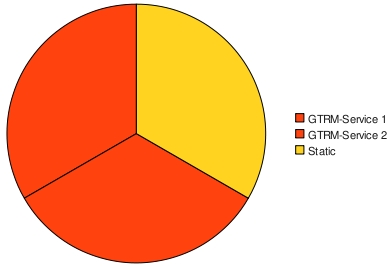
\includegraphics{piechart.jpeg}
    \caption{Pie chart describing how we split up our resources}
    \label{fig:Piechart}
\end{figure}

Using slices one can set a minimum amount of available resources for the applications in the slice. If the applications under a slice/service don’t use all of the resources given to them, the unused resources are free to be used by other slices. Under each slice there can be sub-slices or services dividing the resources further, building a hierarchy in the cgroups folder. The slices in the pie chart above, represent two different sets of applications. The static yellow slice consists of applications that won’t be managed by GTRM and simply will share the resources under this slice according to a predefined setting. Good choices of applications to put here would be some that doesn’t vary much in their resource requirements or some that have very strict hard deadlines. The second slice, the red GTRM slice, consists of applications that will be managed by the GTRM and that might implement SL adaptation. Good choices of applications to put here would be ones that do vary much in their resource requirements and/or can vary its quality in some acceptable way to adapt to its available resources.

All applications that are managed by the GTRM are run as services under the GTRM-slice. A service can, just as a slice, reserve a minimum percentage of allocated resources from it’s parent slice.

In the Pie chart above the static slice would be guaranteed a minimum of \sfrac{1}{3} of the total resources while Service1 and Service2 would be given half of the \sfrac{2}{3} reserved by its parent slice, guaranteeing  them a minimum of \sfrac{1}{3} of the total available resources each.

The resources of the applications running in the GTRM-slice will be managed by the GTRM. Some of the applications will have SL capabilities implemented and some will not. Ideally all applications running in the GTRM-slice should, if it makes sense to the application, have a SL implemented to put the theory into practice. An extension of the project would be to have the entire system managed by the GTRM and have all applications manage their SL. The weight is the parameter that sets how big part of the adaptation that is made by changing the service level contra changing the amount of resources. By using the weight parameter an application can be set to only use resource adaption. However all applications in the gtrm slice must implement calculation of the performance and communication with the RM.


\subsection{.service and .slice files}
The resource split shown in \ref{fig:Piechart} is made by creating a gtrm.slice file in the folder \emph{/etc/systemd/system}:
\subsubsection{gtrm.slice}
\begin{verbatim}
[Unit]

[Slice]
CPUShares=1024
\end{verbatim}
Create the same service files in the same folder:
\subsubsection{gtrm-test.service and gtrm-test2.service}
\begin{verbatim}
[Unit]

[Service]
ExecStart=/mnt/flash/test-gtrm-app 50 10 0 0 0 0.1 0.5 0.04
CPUShares=100
Slice=gtrm.slice
\end{verbatim}

Any application that wants to use the GTRM needs to create such a service file in this folder.
Systemd creates by default a slice that all services will run under unless otherwise specified. Any service file in the \emph{/etc/systemd/system} folder overrides a service file for the 
same application declared somewhere else.




\section{Sequence diagram}
\begin{figure}
    \centering
    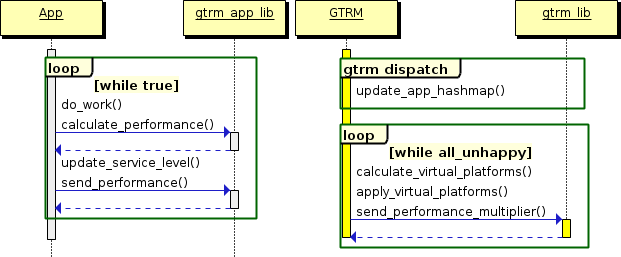
\includegraphics[width=\textwidth]{diag.png}
    \caption{Sequence diagram}
    \label{fig:sdiag}
\end{figure}
The sequence diagram in figure \ref{fig:sdiag} describes the flow of execution throughout the system via pseudo-code. Some functions call that are not relevant have been left out but will be described further below. 

The first important part in the application is the calculation of its performance, the matching function, here called \emph{calculate\_performance()}. The matching function has to be properly calculated or else the application will not be managed correctly. According to this matching function the service level will then be adapted, \emph{update\_service\_level()} and finally the resource manager will be notified by the \emph{send\_performance()} call.

The resource manager part basically consists of two parts that sort of runs in parallel. Upon receiving the performance of an application, the handler or dispatch function corresponding to such an event is executed. In the diagram it is labled as \emph{gtrm\_dispatch}, and its main responsibilities is to read and parse the received message and then update the hash-map which contains the relevant data about the applications being managed. Meanwhile the resource management runs as a part of the main-loop, and it uses the information in the hash-map previously mentioned to calculate the virtual platforms, \emph{calculate\_virtual\_platforms}. These virtual platforms are then used to set the amount of CPUShares which will be given to each application in the call to \emph{apply\_virtual\_platforms}. To get a better service level adaptation, the performance number which depends on how much the virtual platform has been changed is sent to the application \emph{send\_performance\_number}.



\chapter{Use cases}
\label{chp:usecases}

For implementation and testing reasons we came up with the following use-cases. In all the use cases we assume that the static slice is under heavy load so that no extra resources are given to the GTRM-slice. 
\section{Normal mode}
\begin{enumerate}
\item The system runs under good conditions, meaning we have enough resources for all applications and the GTRM-slice can run at maximum SL without any problems.
\item The GTRM and SL adaptation will not drag down performance compared to the old system.
\end{enumerate}
\section{Balancing a high load caused by video streaming}
The applications mentioned here are all on the GTRM-slice.

\begin{enumerate}
\item The camera will film something that causes a high load, for example, a PTZ-camera is moving around or an intense scenery is being filmed.
\item The applications with the worst performance  will adapt and lower their SL (e.g. quality) assuming they have weights setup to do so.
\item The GTRM will increase the resources given to the applications with the worst performance. These resources are taken from other, better performing,  processes on the slice that in turn will lower their SL to accommodate for the change in CPU.
\item When the scenery is “calmer” we will have an overall increase on the SL and the virtual platform will be redistributed.
\item The frame rate will be about the same during the entire procedure.
\end{enumerate}
\section{Balancing a high load caused by other applications}
In this case the static slice starts out not being under full load.
\begin{enumerate}
\item The static slice is giving extra resources to the GTRM-slice, making the applications on the GTRM-slice have a higher SL than they normally would.
\item The resource demand of the applications on the static slice starts to grow. 
\item The SL of the applications on the GTRM-slice will adapt and lower their SL:s (e.g. quality).
\item The static slice is done with the more demanding tasks and starts giving extra resources to the GTRM-slice again. Now we will see an increase in the SL and a redistribution of CPU resources to the applications on the GTRM-slice.
\item The frame rate will be about the same during the entire procedure.
\item The applications in the static slice will run without any issues.
\end{enumerate}
\section{GTRM-slice not running}
\begin{enumerate}
\item No applications are running in the GTRM-slice.
\item The static slice is allowed to use the entire amount of resources if necessary.
\item Some applications on the GTRM-slice starts to run.
\item The GTRM-slice will adjust its SL and virtual platforms as in ‘use case 3’ .
\end{enumerate}

\section{Applications with different weights}
\begin{enumerate}
\item Applications with different weights are running in the GTRM-slice. All applications have a good enough performance which means that no adaptation or resource management is running. 
\item One of the applications performance goes bad.
\item Resource management and SL adaptation for all applications starts.
\item The applications with the higher weights adapts mainly by increasing their cpu, which typically goes faster than adjusting the SL, making them reach a good performance faster. At the same time the applications with lower weights changes more slowly toward a better performance and adapts mainly by lowering their SL.
\item The system reaches a stable point.
\end{enumerate}

\section{System reaches stable point with some bad performances}
\begin{enumerate}
\item A number of applications are running with good performances and no adaptation or resource management is being made.
\item A new application is started with a default SL.
\item Resource manager and SL adaptation is started.
\item The system reaches a stable point where not all applications have a good performance. 
\item The applications that supports SL adaptation will have lowered this as much as possible.
\item The GTRM loop will continue to run. The SL adaptation in the applications will not run if the SL is at minimum and the performance is below the defined boundary or if the SL is at maximum and the performance is above the boundary.
\end{enumerate}

\chapter{Testing}
\label{chp:test}

The end result will be a working prototype that can demonstrate that the system works and what results that can be expected. These are the main aspects that we want to test.
To provide results and to prove that the thesis is valid, thorough testing is required. The main focus of the test is to see if the following can be achieved.
\begin{itemize}
\item Can we keep the FPS we want even during high load of the system.
\item Can we adapt so that other applications can perform well during high loads as well. 
\end{itemize}

The test output consist of logs showing CPU-time for applications along with their service levels, performance and virtual platforms. The CPU-time differ between how much resources are assigned to each application and how much is actually used and it is of interest to see how much they vary if any. The FPS and video quality are other outputs that has to be taken into the result.

It is also desirable to test if the system can fulfill the previously described use cases.

\begin{itemize}

\item The first and simplest case is a camera that is still and filming a scenery which does not change notably. Here it is expected maximal quality of the images since the scene itself does not require a lot of resources. 
\item Next step is to test more complex scenery, for example scenery with a lot of different things going on at the same time. This will stress the video streaming and we want to make sure that if necessary the quality will be reduced in favor for a steady FPS.
\item A moving PTZ-camera will cause a high load when it is moving around. This will cause the whole picture to be redrawn and not partly as when the image is still, and will be the ultimate stress test for the streaming part.
\item By running different test applications that are resource demanding the camera can be tested during intense CPU-loads. Some of the applications will have a linear relationship between computational time and the SL while others will have a non linear one. This matters since the SL adaptation assumes a linear relationship between the SL and the computational time. If the steps in SL are small enough the linear relationship could still be assumed even for non linear ones.
\end{itemize}

\chapter{Results}
\label{chp:results}

\chapter{Conclusion and Further Work}
\label{chp:conclusion}


%\printbibliography  %% Comment if you don't want to use bibtex

\bibliographystyle{plain}
\bibliography{mybib}
\appendix
\chapter{Source Code Overview}
In this section follows an overview of the header and source files used in the system and their attributes.
\section{gtrm\_lib.c/h}
A library which contains various functions used by the resource manager to make various computations and inter process communication.

\subsection{struct rm\_app\_t}
Represents an application being managed and consists of the following fields.
\begin{itemize}
\item tid: Applications PID.
\item vp: Virtual platform.
\item vp\_old: Previous virtual platform.
\item performance: Performance, or matching function of the application.
\item weight: The current "weight" of the application.
\item happy: Indicates if the application is happy with its current performance.
\item sa: Socket Address, used to send back the performance multiplier.
\end{itemize}

\subsection{struct gtrm\_t}
Stores various parameters used by the GTRM.
\begin{itemize}
\item c1: Constant used for computing epsilon, determines how much we will change the virtual platform.
\item c2: Another constant used for computing epsilon similar as c1.
\item iterations: Keeps track of how many iterations the GTRM has run.
\item all\_happy: Used to indicate if we have to make any adjustments to the resource allocations.
\item num\_apps: Total amount of applications that we are managing.
\item prev\_apps: The amount of applications in the previous iteration.
\end{itemize}

\subsection{void gtrm\_char2gtrmstruct(char* str, rm\_app\_t *re)}
Extracts data from a received string and store it as a struct instead. The data sent from an application consists of the PID, performance, weight and if the application is satisfied or not.
\begin{itemize} 
\item str: String to extract data from.
\item re: Struct to hold the extracted data.
\item Return value: None, the result is stored in \emph{re}.
\end{itemize}

\subsection{int gtrm\_send\_performance\_multiplier(double pm, int fd, struct sockaddr *sa)}
Sends a performance multiplier to an application via sockets.
\begin{itemize} 
\item pm: Performance multiplier to send.
\item fd: File descriptor used to send the performance multiplier.
\item sa: Socket address.
\item Return value: Always zero.
\end{itemize}

\subsection{double gtrm\_get\_epsilon(unsigned int iterations, unsigned int offset, double c1, double c2)}
Calculates the constant epsilon used by the resource manager.
\begin{itemize} 
\item iterations: Number of iterations run by the RM.
\item offset: One if there is a difference between currently and previously running applications, zero otherwise.
\item c1: Constant, previously described.
\item c2: Constant, also previously described.
\item Return value: The calculated epsilon or one if this is the first iteration.
\end{itemize}

\subsection{void gtrm\_update\_performance\_multipliers(int gtrm\_fd, Hashmap *gtrm\_apps)}
Calculates, updates and sends the performance multiplier to each application, using the performance, virtual platform and the previous virtual platform for each application.
\begin{itemize} 
\item gtrm\_fd: File descriptor used to send the performance multiplier.
\item gtrm\_apps: Hash-map containing rm\_app\_t structs for each application.
\item Return value: None.
\end{itemize}

\subsection{void gtrm\_write\_log(Hashmap *gtrm\_apps, unsigned int num\_applications)}
Writes information about the resource management to a log file, which can then be used to generate some nice graphs.
\begin{itemize} 
\item gtrm\_apps: Hash-map containing rm\_app\_t structs for each application.
\item num\_applications: Used to make sure we don't try to print an empty hash-map.
\item Return value: None.
\end{itemize}

\section{manager.c/h}
One of the main files in systemd and is for example responsible for inter process communication. The following fields are added to the \emph{Manager} struct in manager.h:
\begin{itemize}
\item gtrm\_socket: String that represent the socket used by GTRM.
\item gtrm\_fd: A file descriptor, which is an integer, for communicating with GTRM.
\item gtrm\_event\_source: Used to determine the source of an event and how this event is supposed to be handled.
\item gtrm\_apps: Hash-map containing all the applications being managed by the GTRM.
\end{itemize}



\subsection{static int manager\_dispatch\_gtrm\_fd(sd\_event\_source *source, int fd, unit32\_t revents, void *userdata)}
Called when we receive the performance of an application.
\begin{itemize}
\item source: source of the event.
\item fd: file descriptor to the event source.
\item revents: Set by the kernel to indicate what event on the file descriptor that triggered the call to this function. In our case it is always the incoming event.
\item userdata: In this case it contains a reference to the manager.
\item Return value: Not used, always zero.
\end{itemize}

\subsection{static int manager\_setup\_gtrm(Manager *m)}
Used to setup the socket, event source and file descriptor for the resource manager. Called from manager\_startup and manager\_reload.
\begin{itemize}
\item m: Reference to the manager.
\item Return value: Zero if function ran correctly, otherwise it is set to the corresponding error number.
\end{itemize}

\subsection{int gtrm\_compute\_virtual\_platforms(Hashmap *apps, gtrm\_t *gtrm\_t)}
Calculates the amount of resources (virtual platform) for an application.
\begin{itemize}
\item apps: The hash-map containing information about the applications being managed.
\item gtrm\_t: Struct with parameters used when calculating the virtual platforms.
\item Return value: Not used, always zero.
\end{itemize}

\subsection{void gtrm\_apply\_virtual\_platforms(Manager* m)}
Computes and applies the amount of CPUShares that each application shall be given.
\begin{itemize}
\item m: Reference to manager, used to get the applications
\item Return value: None.
\end{itemize}

\subsection{int manager\_loop(Manager *m)}
The main loop of the system which continuously calls gtrm\_compute\_virtual\_platforms, gtrm\_apply\_virtual\_platforms and gtrm\_update\_performance\_multipliers if all applications are not satisfied with their performance.
\begin{itemize}
\item m: Reference to manager, used to get the applications.
\item Return value: Exit code of systemd.
\end{itemize}

\subsection{int manager\_set\_cpu\_shares(Manager *m, pid\_t pid, int shares)}
Sets the CPUShares of an application.
\begin{itemize}
\item m: Reference to manager, used to get the applications.
\item pid: Process identifier of the application.
\item shares: Amount of shares we want to set.
\item Return value: Zero if successful, one otherwise.
\end{itemize}

\section{gtrm\_app\_lib.c/h}
These files are used by the applications to get performance, send performance and setup IPC, for example.
In the header file the following structs are defined:
\subsection{struct \_job\_h}
A struct used to represent a job. Applications can have different type of jobs with different deadlines. We only use one type however.
\begin{itemize}
\item id: Identifier to keep track of a job being executed.
\item type: What type of job this is.
\item start\_timestamp: Time when the job was started.
\item end\_timestamp: Time when we were finished with job. The timestamps are used to calculate the total execution time of a job.
\end{itemize}

\subsection{struct \_application\_h}
Each application stores the relevant information in terms of resource management and SL-adaptation in this struct.
\begin{itemize}
\item application\_id: Identifier for an application.
\item jobs: Number of possible job types
\item weight: Determines how to divide the adaptation between the resource manager and service level adaptation.
\item performance\_multiplier: Depends on how the virtual platform has changed and is used for better service level adaptation.
\item total\_jobs: How many jobs that has been launched in total.
\item progress\_jobs: Jobs in progress.
\item completed\_jobs: Total amount of completed jobs.
\item expected\_response\_times: Array of the expected response time for each job type.
\item happy: Indicates if the application is satisfied with its performance or not.
\end{itemize}

\subsection{int gtrm\_lib\_setup\_socket(char* filename)}
Sets up a socket to communicate with the resource manager.
\begin{itemize}
\item filename: The socket needs a file to work, the parameter specifies its path.
\item Return value: Zero, not used.
\end{itemize}

\subsection{void gtrm\_lib\_send\_performance(\_application\_h *h, double performance)}
Sends the performance of an application to the GTRM.
\begin{itemize}
\item h: Struct representing an application.
\item performance: Performance or matching function to send to the GTRM.
\item Return value: None.
\end{itemize}

\subsection{int gtrm\_lib\_set(\_application\_h* a, uint types, uint64\_t* ert)}
Initializes the application struct with job types and their expected response times.
\begin{itemize}
\item a: Struct representing an application.
\item types: Number of different job types.
\item ert: Array of expected response time for each job type.
\item Return value: Exit status of function.
\end{itemize}

\subsection{static int manager\_setup\_gtrm(Manager *m)}
Used to setup the socket, event source and file descriptor for the resource manager. Called from manager\_startup and manager\_reload.
\begin{itemize}
\item m: Reference to the manager.
\item Return value: Zero if function ran correctly, otherwise it is set to the corresponding error number.
\end{itemize}

\subsection{double gtrm\_lib\_get\_performance\_number(\_application\_h* a, int job\_type)}
Calculates the peformance (matching function) by averaging the performance of the last ten jobs of a specified type.
\begin{itemize}
\item a: Struct representing an application.
\item type: Which job type for which we want to calculate the performance.
\item Return value: Applications performance.
\end{itemize}

\subsection{int gtrm\_lib\_update\_performance\_multiplier(\_application\_h *a)}
Receives the performance multiplier computed by the RM.
\begin{itemize}
\item a: Struct for representing the application, and storing the performance multiplier.
\item Return value: Zero, never used.
\end{itemize}

\subsection{int gtrm\_lib\_signalstart(\_application\_h* a, uint type)}
Indicates the start of a job.
\begin{itemize}
\item a: Struct for representing the application.
\item type: Type of the job that is started.
\item Return value: Identifier of the started job.
\end{itemize}

\subsection{int gtrm\_lib\_signalend(\_application\_h* a, uint id)}
Indicates the end of a job.
\begin{itemize}
\item a: Struct for representing the application.
\item id: Identifier of the job that has completed.
\item Return value: Exit status.
\end{itemize}


\end{document}

%KÄLLOR: 
%[sysd] 	http://www.freedesktop.org/wiki/Software/systemd/
%		http://0pointer.de/blog/projects/systemd.html
%[cgropus]	https://www.kernel.org/doc/Documentation/cgroups/cgroups.txt
%[sysd-notify]	http://www.freedesktop.org/software/systemd/man/systemd-notify.html
%[socket]      	http://infohost.nmt.edu/~eweiss/222_book/222_book/0201433079/ch16lev1sec2.html
%[p3367]	http://www.axis.com/files/manuals/um_p3367v_49013_en_1211.pdf
%[m1033]	
%[artpec-4]	http://www.axis.com/corporate/press/se/releases/viewstory.php?case_id=2374
%[gst]		http://gstreamer.freedesktop.org/
%		http://docs.gstreamer.com/display/GstSDK/Tutorials
%[sockets]	http://beej.us/guide/bgnet/output/html/multipage/theory.html
%		http://pic.dhe.ibm.com/infocenter/zvm/v6r2/index.jsp?topic=/com.ibm.zos.r12.cbcpx01/ovsock.htm
%[epoll]	http://en.wikipedia.org/wiki/Epoll

